\documentclass[12pt,letterpaper]{exam}
\usepackage[lmargin=1in,rmargin=1in,tmargin=1in,bmargin=1in]{geometry}
\usepackage{../style/exams}

% -------------------
% Course & Exam Information
% -------------------
\newcommand{\course}{MAT 101: Exam 1}
\newcommand{\term}{Fall -- 2023}
\newcommand{\examdate}{10/11/2023}
\newcommand{\timelimit}{85 Minutes}

\setbool{hideans}{true} % Student: True; Instructor: False

% -------------------
% Content
% -------------------
\begin{document}

\examtitle
\instructions{Write your name on the appropriate line on the exam cover sheet. This exam contains \numpages\ pages (including this cover page) and \numquestions\ questions. Check that you have every page of the exam. Answer the questions in the spaces provided on the question sheets. Be sure to answer every part of each question and show all your work. If you run out of room for an answer, continue on the back of the page --- being sure to indicate the problem number.} 
%\scores
{
\renewcommand{\arraystretch}{2.5}
\begin{table}[H]
\centering
\begin{tabular}{|cccccc|}
\hline
\multicolumn{1}{|c|}{Question} & \multicolumn{1}{c|}{Points} & \multicolumn{1}{c|}{Score} & \multicolumn{1}{c|}{Question} & \multicolumn{1}{c|}{Points} & Score \\ \hline
\multicolumn{1}{|c|}{1} & \multicolumn{1}{c|}{5} & \multicolumn{1}{c|}{} & \multicolumn{1}{c|}{11} & \multicolumn{1}{c|}{5} &  \\ \hline
\multicolumn{1}{|c|}{2} & \multicolumn{1}{c|}{5} & \multicolumn{1}{c|}{} & \multicolumn{1}{c|}{12} & \multicolumn{1}{c|}{5} &  \\ \hline
\multicolumn{1}{|c|}{3} & \multicolumn{1}{c|}{5} & \multicolumn{1}{c|}{} & \multicolumn{1}{c|}{13} & \multicolumn{1}{c|}{5} &  \\ \hline
\multicolumn{1}{|c|}{4} & \multicolumn{1}{c|}{5} & \multicolumn{1}{c|}{} & \multicolumn{1}{c|}{14} & \multicolumn{1}{c|}{5} &  \\ \hline
\multicolumn{1}{|c|}{5} & \multicolumn{1}{c|}{5} & \multicolumn{1}{c|}{} & \multicolumn{1}{c|}{15} & \multicolumn{1}{c|}{5} &  \\ \hline
\multicolumn{1}{|c|}{6} & \multicolumn{1}{c|}{5} & \multicolumn{1}{c|}{} & \multicolumn{1}{c|}{16} & \multicolumn{1}{c|}{5} &  \\ \hline
\multicolumn{1}{|c|}{7} & \multicolumn{1}{c|}{5} & \multicolumn{1}{c|}{} & \multicolumn{1}{c|}{17} & \multicolumn{1}{c|}{5} &  \\ \hline
\multicolumn{1}{|c|}{8} & \multicolumn{1}{c|}{5} & \multicolumn{1}{c|}{} & \multicolumn{1}{c|}{18} & \multicolumn{1}{c|}{5} &  \\ \hline
\multicolumn{1}{|c|}{9} & \multicolumn{1}{c|}{5} & \multicolumn{1}{c|}{} & \multicolumn{1}{c|}{19} & \multicolumn{1}{c|}{5} &  \\ \hline
\multicolumn{1}{|c|}{10} & \multicolumn{1}{c|}{5} & \multicolumn{1}{c|}{} & \multicolumn{1}{c|}{20} & \multicolumn{1}{c|}{5} &  \\ \hline
\multicolumn{2}{|r}{Points:} & \multicolumn{1}{l}{} & \multicolumn{1}{r}{/100} & \multicolumn{2}{l|}{} \\ \hline
\end{tabular}
\end{table}
}
%\bottomline
\newpage

% ---------
% Questions
% ---------
\begin{questions}

% Question 1
\newpage
\question[5] Find the prime factorizations of the following:
	\begin{enumerate}[(a)]
	\item 396
	\item 440
	\end{enumerate}



% Question 2
\newpage
\question[5] Showing all your work, compute the following:
	\begin{enumerate}[(a)]
	\item $\gcd(36, 54)$
	\item $\lcm(36, 54)$
	\end{enumerate}



% Question 3
\newpage
\question[5] Showing all your work, compute the following:
	\begin{enumerate}[(a)]
	\item $\gcd \big(2^{40} \cdot 3^{90} \cdot 5^{30} \cdot 17^5,\; 2^{50} \cdot 3^{80} \cdot 11^{20} \cdot 17^5 \big)$ \par\vspace{0.3cm}
	\item $\lcm \big(2^{40} \cdot 3^{90} \cdot 5^{30} \cdot 17^5,\; 2^{50} \cdot 3^{80} \cdot 11^{20} \cdot 17^5 \big)$
	\end{enumerate}



% Question 4
\newpage
\question[5] Showing all your work and simplifying as much as possible, compute the following:
	\begin{enumerate}[(a)]
	\item $\dfrac{99}{140} - \dfrac{29}{42}$ \par\vspace{0.3cm}
	\item $\dfrac{7}{15} - \dfrac{6}{10} + \dfrac{5}{6}$
	\end{enumerate}



% Question 5
\newpage
\question[5] Showing all your work and simplifying as much as possible, compute the following:
	\begin{enumerate}[(a)]
	\item $\dfrac{20}{66} \cdot \dfrac{117}{15}$ \par\vspace{0.3cm}
	\item $\dfrac{\;\;\dfrac{33}{12}\;\;}{\;\;\dfrac{45}{26}\;\;}$
	\end{enumerate}



% Question 6
\newpage
\question[5] Showing all your work and simplifying as much as possible, convert the given improper fractions to a proper fraction and the given proper fraction to an improper fraction:
	\begin{enumerate}[(a)]
	\item $-\frac{129}{7}$
	\item $-11 \frac{7}{10}$
	\end{enumerate}



% Question 7
\newpage
\question[5] Showing all your work, simplify the following as much as possible: 
	\[
	\dfrac{x^{-5} y^6}{x^3 y^{-2} (x^3 y^5)^{-2}} \left( \dfrac{xy \big( (x^3 y^{-5})^2 \big)^{-4}}{x^0 y^8 (x^{-5} y^6)^{-12}} \right)^0
	\]



% Question 8
\newpage
\question[5] Showing all your work, simplify the following as much as possible: 
	\[
	\sqrt{ \dfrac{9 (a^6 b^5)^{1/3}}{a^{-2} b} }
	\]



% Question 9
\newpage
\question[5] Showing all your work, simplify the following as much as possible:
	\begin{enumerate}[(a)]
	\item $\sqrt{24}$
	\item $\sqrt[3]{24}$
	\end{enumerate}



% Question 10
\newpage
\question[5] Showing all your work and simplifying as much as possible, convert the following decimal number $0.\overline{23}$ to a fraction. 



% Question 11
\newpage
\question[5] Showing all your work and simplifying as much as possible, compute the following:
	\begin{enumerate}[(a)]
	\item $(8 - 6i) - (5 - 9i)$
	\item $\dfrac{1 - 4i}{-4 + 5i}$
	\end{enumerate}



% Question 12
\newpage
\question[5] Showing all your work, compute the following:
	\begin{enumerate}[(a)]
	\item 67\% of 7690
	\item 0.1\% of 4500
	\end{enumerate}



% Question 13
\newpage
\question[5] Showing all your work, compute the following:
	\begin{enumerate}[(a)]
	\item 95 increased by 108\%
	\item 720 decreased by 35\%
	\end{enumerate}



% Question 14
\newpage
\question[5] Given the following course grade components, weights, and student scores, compute the student's course average. 
	\begin{table}[H]
	\centering
	\begin{tabular}{lcc}
	Grade Component & Component Value & Student Grade \\ \hline
	Participation & 5\% & 85\% \\
	Homework & 40\% & 81\% \\
	Project & 15\% & 74\% \\
	Midterm & 15\% & 92\% \\
	Final & 25\% & 86\%
	\end{tabular}
	\end{table}



% Question 15
\newpage
\question[5] Suppose you received the following grades this semester: \par
	\begin{table}[h]
	\centering
	\begin{tabular}{lrc}
	Course & Credits & Grade \\ \hline
	BIO 151: Essentials of Anatomy \& Physiology & 4 & B-- \\
	KIN 202: Motor Development \& Learning & 3 & B+ \\
	SPM 214: Sports Psychology & 3 & A\phantom{-} \\
	CA 219: Modern Movies (1950 -- Present) & 3 & C\phantom{-} \\
	ENG 207: Writing about World Mythology & 3 & A--
	\end{tabular}
	\end{table} \par
Given the following grade values, compute your semester GPA. 
	\begin{table}[h]
	\centering
	\begin{tabular}{lrclr}
	Grade & Values & & Grade & Values \\ \hline
	A & 4.0 & \hspace{1cm} & C+ & 2.3 \\
	A-- & 3.7 & & C & 2.0 \\
	B+ & 3.3 & & C-- & 1.7 \\
	B & 3.0 & & D & 1.0 \\
	B-- & 2.7 & & F & 0
	\end{tabular}
	\end{table} 



% Question 16
\newpage
\question[5] Convert the given decimal number to scientific notation and the given number in scientific notation to a decimal number:
	\begin{enumerate}[(a)]
	\item $1.4567 \cdot 10^2$
	\item $0.0000065$
	\end{enumerate}



% Question 17
\newpage
\question[5] Showing all your work, compute the following:
	\begin{enumerate}[(a)]
	\item 15~quarts to liters [1~quart = 4~cups; 1~cup = 8~fl oz; 29.57~ml = 1~fl oz]
	\item 9.8~m/s$^2$ to feet per square minute [1~m = 3.28084~ft]
	\end{enumerate}



% Question 18
\newpage
\question[5] A lighthouse is located 7~mi due West and 3~mi due South of you. You will walk a straight path to the lighthouse at a rate of 2.5~mph. How long will it take you to walk to the lighthouse? 



% Question 19 
\newpage
\question[5] Find the perimeter and area of the figure below. 
	\[
	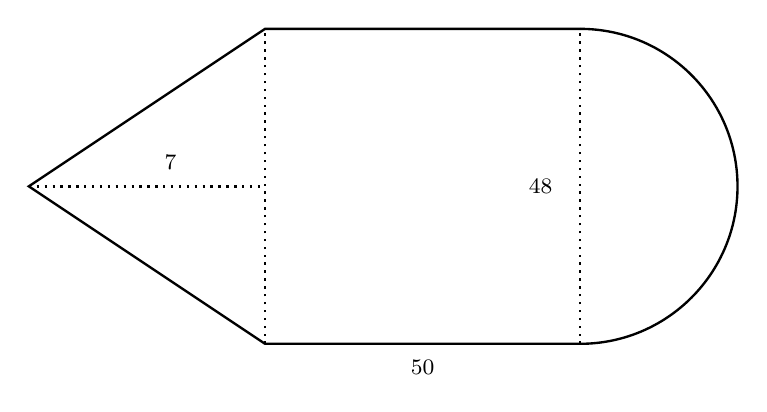
\begin{tikzpicture}
	\draw[line width=0.03cm] (4,-2) -- (0,-2) -- (-3,0) -- (0,2) -- (4,2);
	\draw[line width=0.03cm] (4,-2) arc(-90:90:2);
	
	\draw[line width=0.03cm,dotted] (-3,0) -- (0,0);
	\draw[line width=0.03cm,dotted] (0,-2) -- (0,2);
	\draw[line width=0.03cm,dotted] (4,-2) -- (4,2);
	
	\node at (-1.2,0.3) {\footnotesize 7};
	\node at (2,-2.3) {\footnotesize 50};
	\node at (3.5,0) {\footnotesize 48};
	\end{tikzpicture}
	\]   



% Question 20
\newpage
\question[5] Compute the volume and surface area of the figure below. 
	\[
	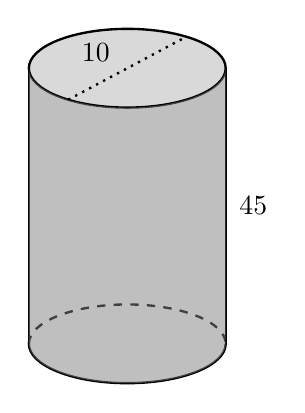
\begin{tikzpicture}
	\draw[line width= 0.03cm,fill=gray!30] (0,3.5) ellipse (1.25 and 0.5);	% Top
	\draw[line width= 0.03cm] (-1.25,3.5) -- (-1.25,0); % Left Side
	\draw[line width= 0.03cm] (1.25,0) -- (1.25,3.5);  % Right Side
	\draw[line width= 0.03cm] (-1.25,0) arc (180:360:1.25 and 0.5); % Bottom 
	\draw[line width= 0.03cm, dashed] (-1.25,0) arc (180:360:1.25 and -0.5); % Bottom Dotted
	\fill[gray,opacity=0.5] (-1.25,3.5) -- (-1.25,0) arc (180:360:1.25 and 0.5) -- (1.25,3.5) arc (0:180:1.25 and -0.5); % Gray Fill
	
	\draw[line width= 0.03cm,dotted] (-0.75,3.1) -- (0.75,3.9); % Top Dotted
	
	% Labels
	\node at (-0.4,3.7) {10};
	\node at (1.6,1.75) {45};
	\end{tikzpicture}
	\]


\end{questions}
\end{document}